%&pdflatex

\documentclass[12pt]{article}

\usepackage[spanish, es-tabla]{babel}
\usepackage{enumerate}
\usepackage{lscape}
\usepackage{vmargin}
\usepackage{pdfpages}
\usepackage{fancyhdr}
\usepackage{graphicx}
\usepackage{float}
\usepackage{titlesec}
\usepackage[bottom]{footmisc}
\usepackage[hidelinks]{hyperref}
\usepackage{listings}
\usepackage{color}
\usepackage{colortbl}
\usepackage{xcolor}
\usepackage{amsmath}
\usepackage{array}
\usepackage{svg}
\usepackage{pgfgantt}
\usepackage[T1]{fontenc}
\usepackage[sfdefault]{AlegreyaSans} %% Option 'black' gives heavier bold face
%% The 'sfdefault' option to make the base font sans serif
\renewcommand*\oldstylenums[1]{{\AlegreyaSansOsF #1}}


%*******************************************************************************
\extrarowheight = -0.3ex
\renewcommand{\arraystretch}{2.25}
\setpapersize{A4}
\hypersetup{
    colorlinks=true,
    linkcolor=blue,
    urlcolor=purple,
    citecolor=black, 
    linktocpage=true,
}
\definecolor{gray95}{gray}{.95}
\definecolor{gray75}{gray}{.75}
\definecolor{barblue}{RGB}{153,204,254}
\definecolor{groupblue}{RGB}{51,102,254}
\definecolor{linkred}{RGB}{165,0,33}
\lstset{
    frame=Ltb,
    framerule=0pt,
     aboveskip=0.5cm,
     framextopmargin=3pt,
     framexbottommargin=3pt,
     framexleftmargin=0.4cm,
     framesep=0pt,
     rulesep=.4pt,
     backgroundcolor=\color{gray95},
     rulesepcolor=\color{cyan},
     %
     stringstyle=\ttfamily,
     showstringspaces = false,
     basicstyle=\small\ttfamily,
     commentstyle=\color{cyan},
     keywordstyle=\bfseries\color{purple},
     %
     numbers=left,
     numbersep=15pt,
     numberstyle=\small,
     numberfirstline = false,
     breaklines=true,
}

%minimizar fragmentado de listados
\lstnewenvironment{listing}[1][]
   {\lstset{#1}\pagebreak[0]}{\pagebreak[0]}


\lstdefinestyle{C}
   {
       language=C++,
   }

\lstdefinestyle{python}
    {
        language=Python,
    }

\setcounter{secnumdepth}{4}
%*******************************************************************************
%   Adding a new level of section --> subsubsubsection
%******************************************************************************
\titleclass{\subsubsubsection}{straight}[\subsection]

\newcounter{subsubsubsection}[subsubsection]
\renewcommand\thesubsubsubsection{\thesubsubsection.\arabic{subsubsubsection}}
\renewcommand\theparagraph{\thesubsubsubsection.\arabic{paragraph}} % optional; useful if paragraphs are to be numbered

\titleformat{\subsubsubsection}
  {\normalfont\normalsize\bfseries}{\thesubsubsubsection}{1em}{}
\titlespacing*{\subsubsubsection}
{0pt}{3.25ex plus 1ex minus .2ex}{1.5ex plus .2ex}

\makeatletter
\renewcommand\paragraph{\@startsection{paragraph}{5}{\z@}%
  {3.25ex \@plus1ex \@minus.2ex}%
  {-1em}%
  {\normalfont\normalsize\bfseries}}
\renewcommand\subparagraph{\@startsection{subparagraph}{6}{\parindent}%
  {3.25ex \@plus1ex \@minus .2ex}%
  {-1em}%
  {\normalfont\normalsize\bfseries}}
\def\toclevel@subsubsubsection{4}
\def\toclevel@paragraph{5}
\def\toclevel@paragraph{6}
\def\l@subsubsubsection{\@dottedtocline{4}{7em}{4em}}
\def\l@paragraph{\@dottedtocline{5}{10em}{5em}}
\def\l@subparagraph{\@dottedtocline{6}{14em}{6em}}
\makeatother

\setcounter{secnumdepth}{4}
\setcounter{tocdepth}{4}

%*****************************************************************************

\begin{document}

  \begin{titlepage}
    \centering
   {\bfseries\Large Universidad Carlos III de Madrid \par}
    \vspace{5cm}
    {\scshape\Huge Informe de la tercera práctica de laboratorio\par}
    \vspace{2cm}
    {\itshape\Large Diseño de circuitos electrónicos para comunicaciones}
    \vfill
    {\Large Autores: \par}
    \vspace{1cm}
    {\Large Markel Serrano y Daniel Theran}
    \vfill
    {\Large 19 de diciembre del 2022 \par}
  \end{titlepage}

  \section{Apartado 1: cálculos teóricos}

    \paragraph*{}
    En este apartado se pretende caracterizar el VCO y el contador utilizando como guía la data sheet que nos proporciona el vendedor. En concreto se busca encontrar cuál es la $K_{VCO}$ y la $K_{VCF}$
    (ganancia de frecuencia en rad/s/v y ganancia del detector de fase en V/rad/s respectivamente) para posteriormente contrastar los resultados teóricos con los experimentales que se mencionan en el apartado siguiente. 

    \paragraph*{}
    Primero revisamos hoja de especificaciones del PLL \textbf{CD4046} \footnote{Data sheet disponible en: \href{https://www.floka.com/cmos/pdf/4046.pdf}{https://www.floka.com/cmos/pdf/4046.pdf}}
    y vemos cual es el valor máximo y mínimo de frecuencia a la que puede funcionar así como las tensiones correspondientes a dichos valores. De la misma obtenemos que cuando el PLL se alimenta con 
    0 V, entonces estamos funcionando a la frecuencia mínima que es también 0 Hz; y cuando lo alimentamos con VDD = 5 V (la tensión de alimentación del esquema), entonces la frecuencia de funcionamiento 
    es 100 kHz.
  
    \paragraph*{}
    Con estos datos podemos sacar que la pendiente y por lo tanto la ganancia $K_{VCO} = 100 kHz/5 V$ o lo que en rad/v será $K_{VCO} = 2\pi·20 rad/V$. 

    \paragraph*{}
    Lo siguiente a calcular es la ganancia $K_{VCF}$ que corresponde con la característica del detector de fase, para ello vamos a la hoja de especificaciones del \textbf{74HCT93} y vemos que al tratarse de un XOR y que ademas 
    se está alimentando a 5V, tenemos entonces que el $K_{VCF} = 5/\pi V/rad$. 

    \paragraph*{}
    Con estos dos valores podemos entonces calcular la función de transferencia teniendo en cuenta que tenemos un filtro RC: 
  
    \begin{center} \label{ec:transfer}
          $\frac{\phi_O}{\phi_r}$ = $\frac{K_{VCO}·K_{VCF}·w_c}{s^2 + s·w_c + K_{VCO}·K_{VCF}·\frac{w_c}{N}}$
    \end{center}
    
     
    Donde: 
    \begin{itemize}
      \item $w_c = \frac{1}{RC}$
      \item $N = f_0/f_{ref} = 16$ 
    \end{itemize}
  
  \paragraph*{}
  Con la función de transferencia obtenida, se procede a realizar su representación en un diagrama de bode con la ayuda de Matlab, dando como resultado la siguiente figura:
  
  \begin{figure}[H]
    \centering
    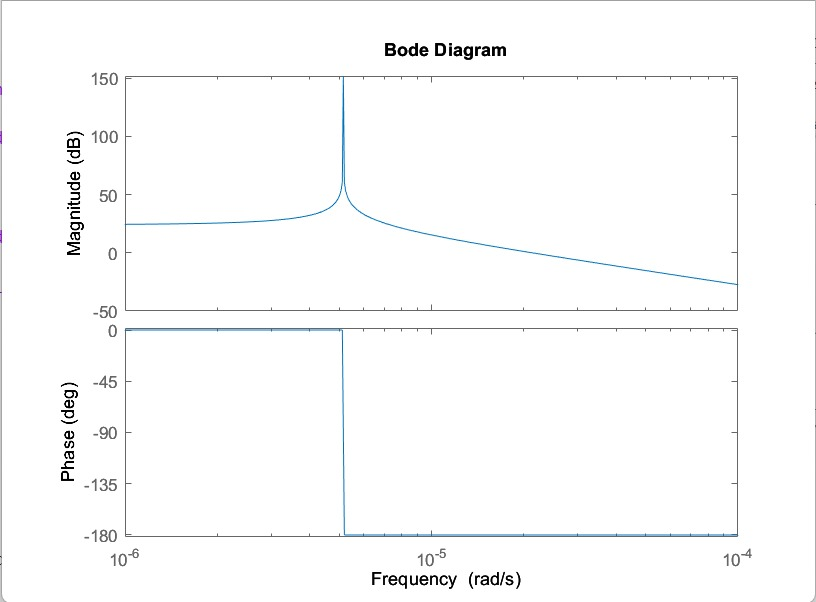
\includegraphics[width=1\linewidth]{img/BODE.jpeg}
    \caption{Diagrama de Bode de la función de transferencia teórica.}%
    \label{fig:bodeteo}
  \end{figure}

  \paragraph*{}
  Se puede observar que ancho de banda es bastante estrecho, lo cual tiene sentido pues el rango de frecuencias en las que engancha la frecuencia de referencia varían entorno 
  a 2 kHz, como se mencionará mas adelante. 
  
  \section{Apartado 2: resultados experimentales}

  \paragraph*{}
  Una vez realizado el montaje del circuito tal y como se indica en el informe, se obtienen, tomando los valores con el osciloscopio tal y como se indica en el informe, para un margen de fijado de 1.32 a 3.29 kHz de frecuencia
  de referencia, los siguientes valores para la salida en frecuencia de VCO, la amplitud de dicha señal y el desfase entre ambas:

\vspace*{1.0cm}

    \begin{table}[H]
      \begin{center}
          \begin{tabular}{| c | c | c | c |}
              \hline
              \rowcolor{black}
              \textcolor{white}{$F_{ref}$ (kHz)} & \textcolor{white}{$F_{VCO}$ (kHz)} & \textcolor{white}{$\Delta \phi$ ($\mu$ s)} & \textcolor{white}{$V_{VCO}$ (V)}\\ \hline
              1.11 & 15.6 & 172 &  2.12\\ \hline
              1.511 & 23.8 & 144 &  2.35\\ \hline
              1.911 & 29.4 & 124 &  2.61\\ \hline
              2.36 & 35.7 & 114 & 2.91\\ \hline
              2.901 & 41.7 & 102 &  3.27\\ \hline
              3.142 & 47.2 & 100 & 3.44\\ 
              \hline 
          \end{tabular}
          \caption{Tabla de resultados reales de la práctica}
          \label{tab:resul_r}
      \end{center}
    \end{table}

  \paragraph*{}
    A muestra de ejemplo, se han tomado como muestra para el informe las frecuencias de referencia de 1.11 kHz y 2.36 kHz, para las que se obtiene
    las siguientes señales de entrada y salida:

    \begin{figure}[H]
      \centering
      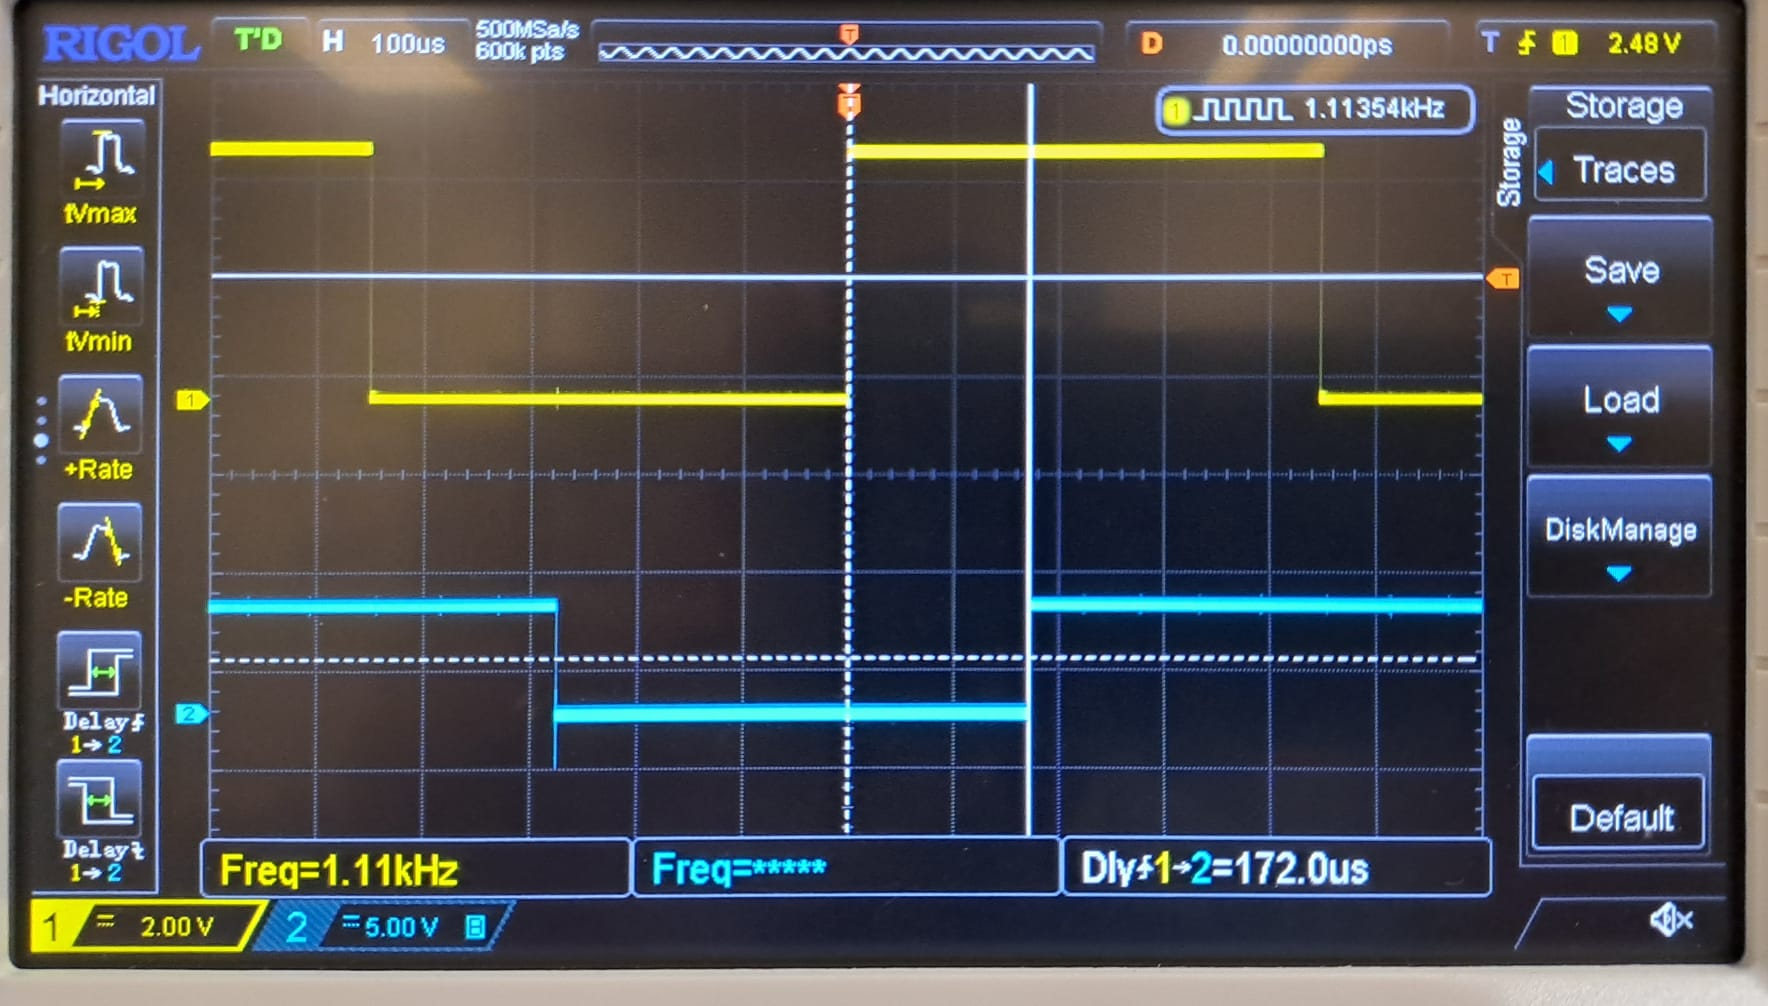
\includegraphics[width=1\linewidth]{img/1khz.jpeg}
      \caption{Señales para 1.11 kHz}%
      \label{fig:1khz}
    \end{figure}
    \paragraph*{}
   
    \begin{figure}[H]
      \centering
      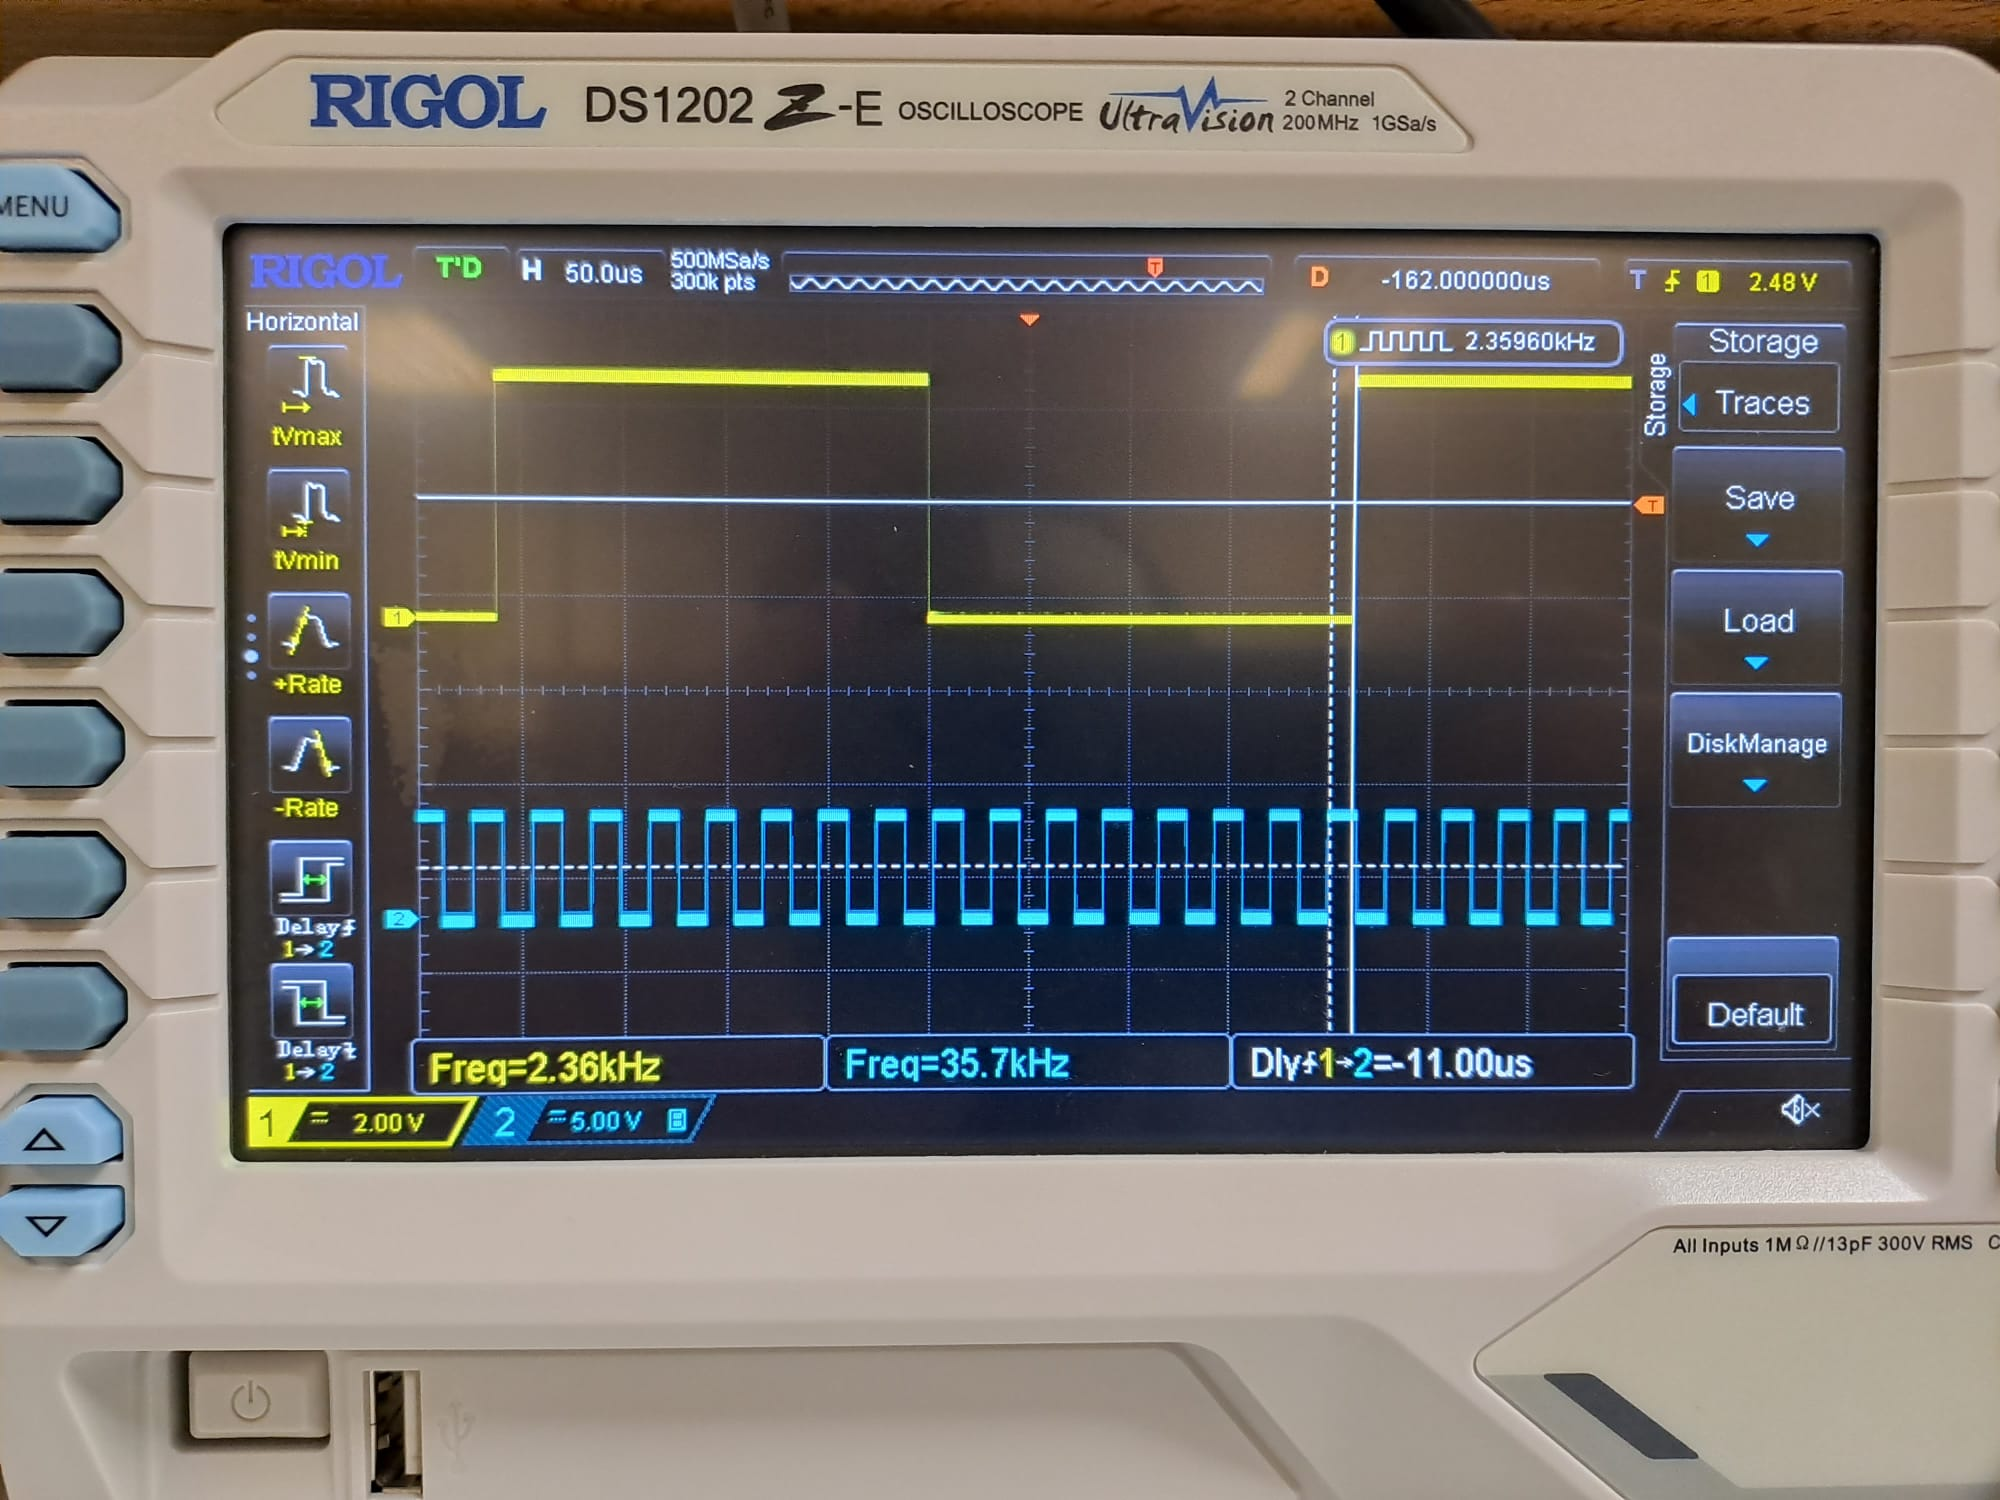
\includegraphics[width=1\linewidth]{img/2khz.jpeg}
      \caption{Señales para 2.36 kHz}%
      \label{fig:2khz}
    \end{figure}


    \paragraph*{}
   Una vez medidos los anteriores valores, podemos situar los distintos puntos encontrados para medir en dos gráficas distintas la frecuencia de salida VCO frente
   a la tensión VCO y la gráfica característica del detector de fase, que muestra la relación entre las dos señales de entrada y de salida (es decir, el desfase entre ambas)
   y la ganancia en tensión que introduce el circuito, es decir, la tensión VCO.
    

    \begin{figure}[H]
      \centering
      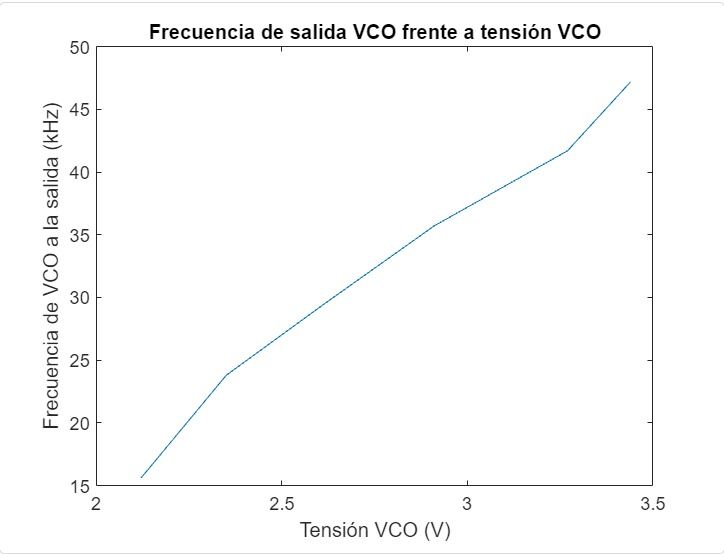
\includegraphics[width=1\linewidth]{img/grafica1.jpeg}
      \caption{Gráfica de relación entre frecuencia VCO y tensión VCO}%
      \label{fig:grafica1}
    \end{figure}

    \paragraph*{}
    Esta primera gráfica muestra la relación entre la frecuencia introducida por el circuito y la amplitud correspondiente. Por tanto, la pendiente de la recta obtenida
para esta gráfica nos muestra la ganancia en frecuencia introducida por el circuito. Así, mediante la ecuación:

 % \paragraph*{}
  \begin{center}
    $K_{VCO} = \frac{F_{VCO2} - F_{VCO1}}{V_{VCO2} - V_{VCO1}}$
  \end{center}
    
 % \paragraph*{}
  Obtenemos una ganancia de frecuencia de 19.45. Hay que remarcar que, debido a los errores de medición y a que la recta no ha sido representada estadísticamente sino como
  una gráfica que une los puntos obtenidos,
  el error en el cálculo de la pendiente es de una magnitud notable.

    \begin{figure}[H]
      \centering
      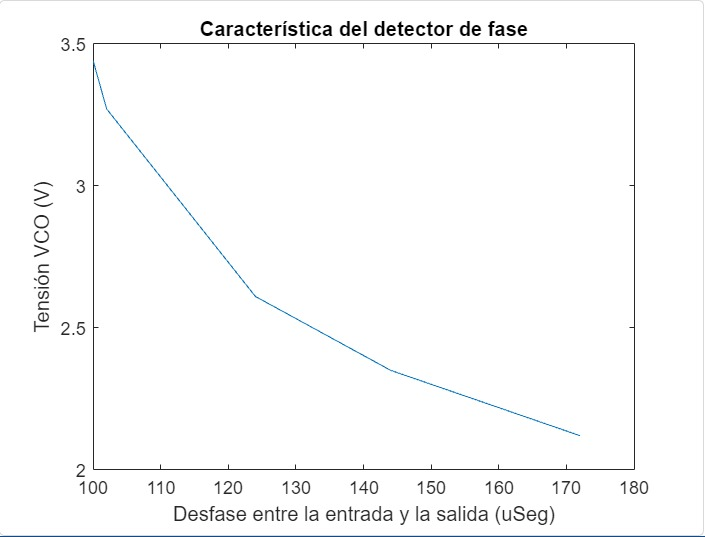
\includegraphics[width=1\linewidth]{img/grafica2.jpeg}
      \caption{Gráfica característica del detector de fase}%
      \label{fig:grafica2}
    \end{figure}
    
    \paragraph*{}
    La segunda gráfica muestra la relación entre la amplitud introducida por el circuito y los desfases entre la señal de entrada y salida. Por tanto, la pendiente de la recta obtenida
para esta gráfica nos muestra la característica del detector de fase. Así, mediante la ecuación:

 % \paragraph*{}
  \begin{center}
    $K_{VCF} = \frac{V_{VCO2} - V_{VCO1}}{\Delta\phi_{2} - \Delta\phi_{1}}$
  \end{center}
    
 % \paragraph*{}
  Obtenemos una magnitud característica de $\frac{9.9}{\pi}$ V/rad, tomando el desfase, que en la tabla aparece representado en microsegundos, en radianes. Debe señalarse que se cometen 
  los mismos errores en el cálculo que para el anterior caso.

  \paragraph*{}
  Con los resultados obtenidos y utilizando la misma función de transferencia (ec. \ref{ec:transfer}), obtenemos el siguiente diagrama de bode en Matlab:
  
  \begin{figure}[H]
    \centering
    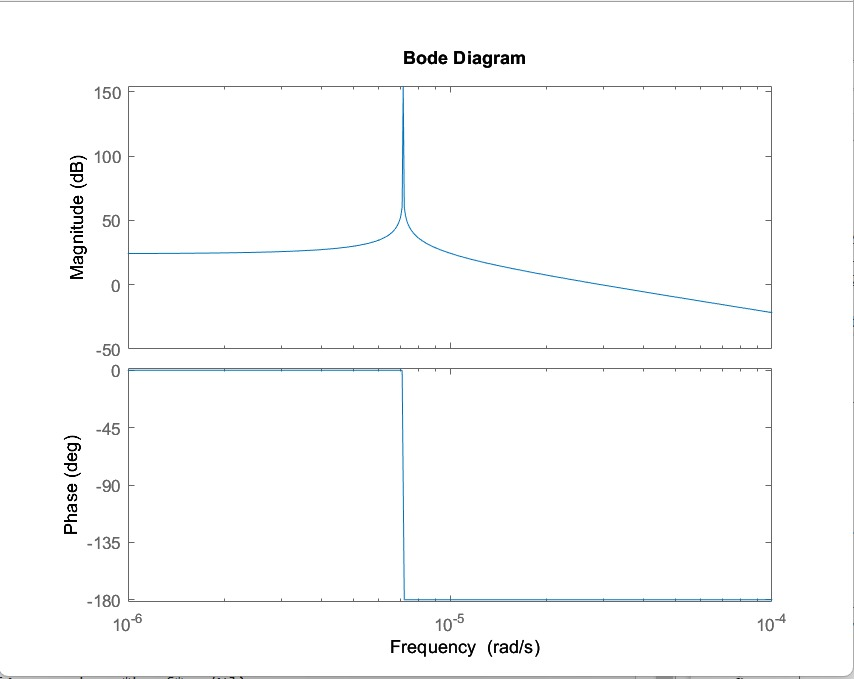
\includegraphics[width=1\linewidth]{img/bode2.jpeg}
    \caption{Diagrama de Bode de la función de transferencia experimental}%
    \label{fig:bodeex}
  \end{figure}
  
  \paragraph*{}
  Como podemos observar, el diagrama de bode experimental es muy similar al real salvo un desplazamiento de la frecuencia central del mismo. 
  

  \section{Apartado 3: resultados conclusiones}
  
  \paragraph*{}
  Como conclusión, se puede observar que el circuito experimental alcanza los mismos resultados que los obtenidos mediante los resultados
  calculados teóricamente. No obstante, hay que realizar algunos comentarios.
  
  \paragraph*{}
  La ganancia del detector de fase obtenida experimentalmente es el doble que la obtenida en el apartado teórico. Esto se debe a que la frecuencia 
  de referencia para la que se consigue fijar una señal VCO estable es aproximadamente 2.5 kHz, con un margen de 1.1 kHz a 3.29 kHz, como se ha mencionado
  anteriormente, cuando lo esperado experimentalmente eran entre 5 y 7 kHz. Dado que el montaje ha sido verificado varias veces y los resultados son 
  coherentes con el diseño del circuito, aunque los valores de la ganancia de detector de fase y frecuencias de referencia sean menores se han dado
  por válidas, considerando este desvío como un problema debido a los componentes empleados, sin afectar así al desarrollo de la práctica.

    


\end{document}